% !TEX program = lualatex
% Compile from 2026/week14; figures are generated by make_figures.py.
\documentclass[12pt,aspectratio=43]{beamer}
% Shared Beamer design. Load after \documentclass using \input.
% Engine: LuaLaTeX. Fonts: UD Digi Kyokasho N (regular/bold), Arial.
\usepackage{luatexja-fontspec}
\setmainjfont[BoldFont={UD Digi Kyokasho N Bold}]{UD Digi Kyokasho N}
\setsansjfont[BoldFont={UD Digi Kyokasho N Bold}]{UD Digi Kyokasho N}
\setmonojfont[BoldFont={UD Digi Kyokasho N Bold}]{UD Digi Kyokasho N}
% Liberation Sans keeps the layout usable on systems without Arial.
\IfFontExistsTF{Arial}{
  \setmainfont{Arial}
  \setsansfont{Arial}
  \setmonofont{Arial}
}{
  \setmainfont{Liberation Sans}
  \setsansfont{Liberation Sans}
  \setmonofont{Liberation Sans}
}
\renewcommand{\kanjifamilydefault}{\gtdefault}

% Typeset mathematics with a dedicated TeX math font, independent of Arial.
\usefonttheme{professionalfonts}
\usepackage[mathrm=sym]{unicode-math}
\setmathfont{Latin Modern Math}
\setoperatorfont{\symup}

\definecolor{courseblue}{HTML}{4472C4}
\definecolor{ruleblue}{HTML}{8FAADC}
\setbeamercolor{normal text}{fg=black,bg=white}
\setbeamercolor{structure}{fg=courseblue}
\setbeamercolor{frametitle}{fg=black,bg=white}
\setbeamercolor{title banner}{fg=white,bg=courseblue}
\setbeamerfont{frametitle}{size=\fontsize{18}{22}\selectfont,series=\mdseries}
\setbeamerfont{quote}{shape=\upshape}
\setbeamersize{text margin left=9mm,text margin right=9mm}
\setbeamertemplate{navigation symbols}{}
\setbeamercolor{page number}{fg=gray,bg=white}
\setbeamertemplate{footline}{%
  \begin{beamercolorbox}[wd=\paperwidth,ht=2.5mm,dp=1.5mm]{page number}
    \hfill{\fontsize{8}{9}\selectfont
      \ifnum\value{framenumber}>0
        \insertframenumber\,/\,\inserttotalframenumber
      \fi}\hspace*{3mm}
  \end{beamercolorbox}}
\setbeamertemplate{headline}{%
  \hfill\textcolor{gray}{\fontsize{6}{7}\selectfont
    \hypersetup{linkcolor=gray}% Keep Beamer's title links in the header color.
    \ifnum\value{framenumber}=0 \insertshortdate\enspace\fi
    \insertshorttitle\space\insertshortsubtitle}\hspace{2mm}\vspace{1.5mm}}
\setbeamertemplate{frametitle}{%
  \vspace{2mm}\centering\insertframetitle\par
  \vspace{-1mm}{\color{ruleblue}\rule{.44\paperwidth}{.5pt}}\par
  \vspace{2mm}}
\setbeamercolor{itemize item}{fg=courseblue}
\setbeamercolor{itemize subitem}{fg=black}
\setbeamercolor{itemize subsubitem}{fg=black}
\setbeamertemplate{itemize item}{\textbullet}
\setbeamertemplate{itemize subitem}{\textnormal{-}}
\setbeamertemplate{itemize subsubitem}{\textnormal{-}}
\setlength{\parskip}{.45em}
\hypersetup{colorlinks=true,urlcolor=courseblue}

% Use \titlepage inside a [t,noframenumbering] frame. The background extends
% 1 mm past both page edges to avoid hairline gaps in PDF viewers.
\setbeamertemplate{title page}{%
  \vspace{2mm}
  \begin{beamercolorbox}[wd=\paperwidth,ht=43mm,dp=13mm,colsep*=1mm,center]{title banner}
    {\fontsize{32}{40}\selectfont\inserttitle\par}
    \vspace{2mm}
    {\fontsize{20}{24}\selectfont\insertsubtitle\par}
  \end{beamercolorbox}
  \vspace{10mm}
  \hfill\insertauthor
}

\graphicspath{{figures/}}
\usepackage{listings}
\usepackage{upquote}
\IfFontExistsTF{Consolas}{\newfontfamily\codefont{Consolas}}{\newfontfamily\codefont{Liberation Mono}}
\definecolor{codevalue}{HTML}{7A3E9D}
\definecolor{codebuiltin}{HTML}{006DB0}
\definecolor{codestring}{HTML}{267348}
\newcommand{\code}[1]{{\codefont #1}}
\lstdefinestyle{python}{
  language=Python,
  basicstyle=\codefont\fontsize{12}{14}\selectfont,
  keywordstyle=\color{codebuiltin},
  stringstyle=\color{codestring},
  showstringspaces=false,
  columns=fullflexible,
  keepspaces=true,
  upquote=true,
  tabsize=4,
  breaklines=false,
  backgroundcolor=\color{black!4},
  frame=single,framerule=0pt,framesep=1.7mm,
  xleftmargin=1.7mm,xrightmargin=1.7mm,
  aboveskip=1mm,belowskip=0.5mm,
  literate=*{0}{{{\color{codevalue}0}}}1
    {1}{{{\color{codevalue}1}}}1 {2}{{{\color{codevalue}2}}}1
    {3}{{{\color{codevalue}3}}}1 {4}{{{\color{codevalue}4}}}1
    {5}{{{\color{codevalue}5}}}1 {6}{{{\color{codevalue}6}}}1
    {7}{{{\color{codevalue}7}}}1 {8}{{{\color{codevalue}8}}}1
    {9}{{{\color{codevalue}9}}}1
}
\lstset{style=python}
\setbeamercolor{lesson note}{fg=black,bg=courseblue!9}
\newenvironment{lessonbox}
  {\begin{beamercolorbox}[wd=\linewidth,sep=1.5mm]{lesson note}}
  {\end{beamercolorbox}\par}

\title{計算物理学B}
\subtitle{第十四回：根の探索}
\author{野垣 康介、藤本 悠輝}
\date{2027/2/2}
\hypersetup{pdftitle={計算物理学B 第十四回：根の探索},pdfauthor={野垣 康介、藤本 悠輝}}

\begin{document}

\begin{frame}[t,noframenumbering]
  \titlepage
\end{frame}

\begin{frame}{講義予定}
  \setlength{\parskip}{0pt}
  2026年度 第2学期（火曜3限）
  \par\vspace{2mm}
  \begingroup\centering
    \renewcommand{\arraystretch}{1.05}
    \begin{tabular}{@{}l@{\hspace{2mm}}l@{\hspace{4mm}}l@{\hspace{2mm}}l@{}}
      10/6 & 四則演算 & 12/8 & モンテカルロ1 \\
      10/27 & 制御文（for, if） & 12/15 & モンテカルロ2 \\
      11/6（金） & 関数 & 12/22 & 微分方程式1 \\
      11/10 & 配列（NumPy） & 1/12 & 微分方程式2 \\
      11/17 & 可視化（matplotlib） & 1/19 & 偏微分方程式1 \\
      11/24 & 数値微分 & 1/26 & 偏微分方程式2 \\
      12/1 & 数値積分 & 2/2 & \textcolor{courseblue}{\textbf{根の探索}} \\
      \multicolumn{2}{c}{\small 〜中間レポート〜} &
      \multicolumn{2}{c}{\small 〜期末レポート〜}
    \end{tabular}\par
  \endgroup
  \vspace{2mm}
  {\small \textcolor{courseblue}{10/20は出張で休講。} 11/6（金）は火曜授業の振替。\par}
\end{frame}

\begin{frame}{授業で使うリンク}
  \begin{itemize}
    \setlength{\itemsep}{3mm}
    \item Google Colab：{\small\url{https://colab.research.google.com/?hl=ja}}
    \item 講義資料（GitHub）：{\small\url{https://github.com/nogaki/Computational_Physics_B}}
    \item 今週のノートブック：\code{2026/week14/week14.ipynb}
    \item 今週のPDF：\code{2026/week14/slide.pdf}
  \end{itemize}
\end{frame}

\begin{frame}[t]{GitHubからColabへ}
  \begin{enumerate}
    \setlength{\itemsep}{4mm}
    \item GitHubで\code{2026/week14/week14.ipynb}を開き、URLをコピーする。
    \item Colabの「ファイル」→「ノートブックを開く」→「GitHub」を選ぶ。
    \item URLを貼り付けて検索し、Notebookを開く。
  \end{enumerate}
  \vspace{3mm}
  \begin{lessonbox}
    \textbf{「ドライブにコピーを保存」を実行する}\par
    \small 開いただけでは自分のGoogle Driveに保存されない。編集前にコピーを作る。
  \end{lessonbox}
\end{frame}

\begin{frame}[t]{方程式の根を数値的に求める}
  方程式\(f(x)=0\)の解を探す。
  \begin{itemize}
    \item 関数の値を調べ、根がある区間や次の近似値を選ぶ。
    \item 二分法は区間を確実に縮める。
    \item Newton法・割線法は近くで速く収束することがある。
    \item 固定点反復は\(x=g(x)\)の形で解を求める。
  \end{itemize}
  \vfill
  \begin{lessonbox}
    近似解を得た後は、\(|f(x)|\)を計算して方程式をどれだけ満たすか確かめる。
  \end{lessonbox}
\end{frame}

\begin{frame}[t]{二分法：区間を半分にする}
  \(a<b\)で関数値の符号が反対なら、連続な\(f\)は区間内に少なくとも1つ根をもつ。
  \[
    f(a)f(b)<0.
  \]
  中点\(m=(a+b)/2\)を計算し、符号が変わる半区間だけを残す。
  \begin{itemize}
    \item 繰り返すたびに区間幅が半分になる。
    \item 単調性は必要ない。連続性と符号変化が必要。
    \item 区間に複数の根があれば、そのうちの1つを探す。
  \end{itemize}
\end{frame}

\begin{frame}[t]{二分法：更新と誤差}
  \begin{enumerate}
    \item 端点で\(f(a)f(b)<0\)を確認する。
    \item 中点\(m=(a+b)/2\)を計算する。
    \item \(f(m)=0\)なら終了。そうでなければ符号変化を保つ半区間を選ぶ。
    \item 区間幅または残差が許容値以下になるまで繰り返す。
  \end{enumerate}
  \[
    b_n-a_n=\frac{b_0-a_0}{2^n}.
  \]
  \small 区間幅が許容誤差になれば、区間内の根までの距離も抑えられる。
\end{frame}

\begin{frame}[t]{二分法とNewton法の幾何}
  \centering
  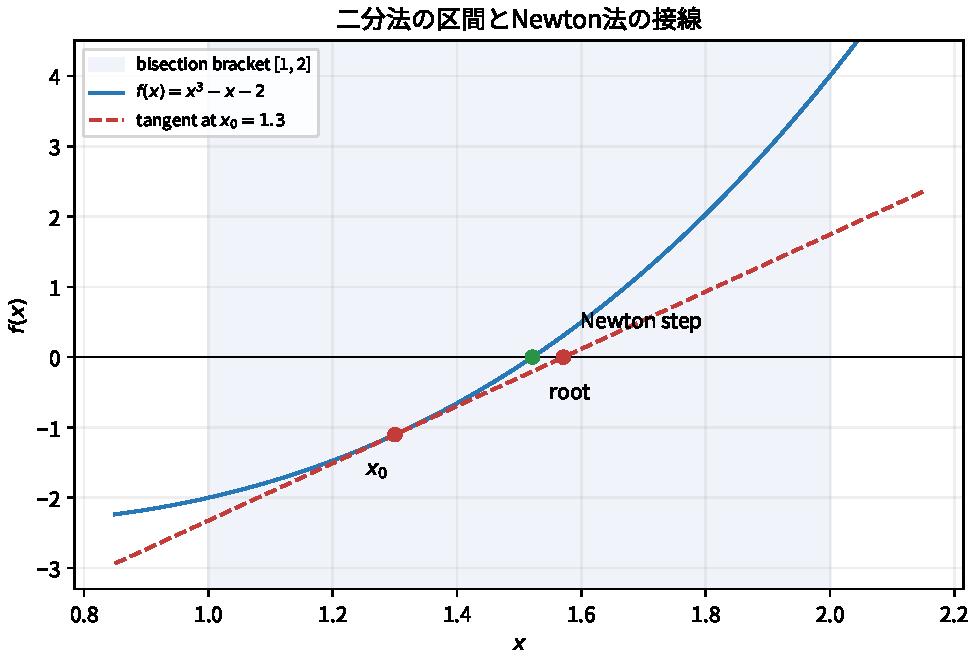
\includegraphics[width=.75\linewidth,height=51mm,keepaspectratio]{root_geometry.pdf}
  \par\small \(f(x)=x^3-x-2\)、二分法の初期区間\([1,2]\)。Newton法は\(x_0=1.3\)の接線と\(x\)軸の交点を次の値にする。
\end{frame}

\begin{frame}[t]{Newton法：接線による更新}
  \(x_n\)の近くでTaylor展開して一次の項まで残す。
  \[
    f(x_n+\delta)\simeq f(x_n)+f'(x_n)\delta.
  \]
  接線が\(x\)軸と交わる点を次の近似にする。
  \[
    x_{n+1}=x_n-\frac{f(x_n)}{f'(x_n)}.
  \]
  \begin{itemize}
    \item 近似が根に近く、単根なら二次収束が期待できる。
    \item 初期値と導関数が必要。
  \end{itemize}
\end{frame}

\begin{frame}[t]{Newton法の注意点}
  \begin{itemize}
    \item \(f'(x_n)=0\)では更新できない。
    \item 導関数が小さいと、一歩が大きくなり区間から離れることがある。
    \item 初期値によっては発散したり、別の根へ向かったりする。
    \item 最大反復回数を設け、残差とステップ幅を確かめて止める。
  \end{itemize}
  \vspace{3mm}
  \begin{lessonbox}
    \(|x_{n+1}-x_n|\)が小さくても、\(|f(x_{n+1})|\)が大きければ収束とはみなさない。
  \end{lessonbox}
\end{frame}

\begin{frame}[t]{割線法：導関数を差分で近似}
  Newton法の導関数を2点の傾きで置き換える。
  \[
    f'(x_n)\simeq\frac{f(x_n)-f(x_{n-1})}{x_n-x_{n-1}}.
  \]
  よって
  \[
    x_{n+1}=x_n-f(x_n)\frac{x_n-x_{n-1}}{f(x_n)-f(x_{n-1})}.
  \]
  \begin{itemize}
    \item 導関数を解析的に用意せずに済む。
    \item 初期値を2つ使う。符号変化の区間を保つ方法ではない。
    \item 分母が0に近い場合、更新が大きくなりうる。
  \end{itemize}
\end{frame}

\begin{frame}[t]{同じ関数で残差を比べる}
  \centering
  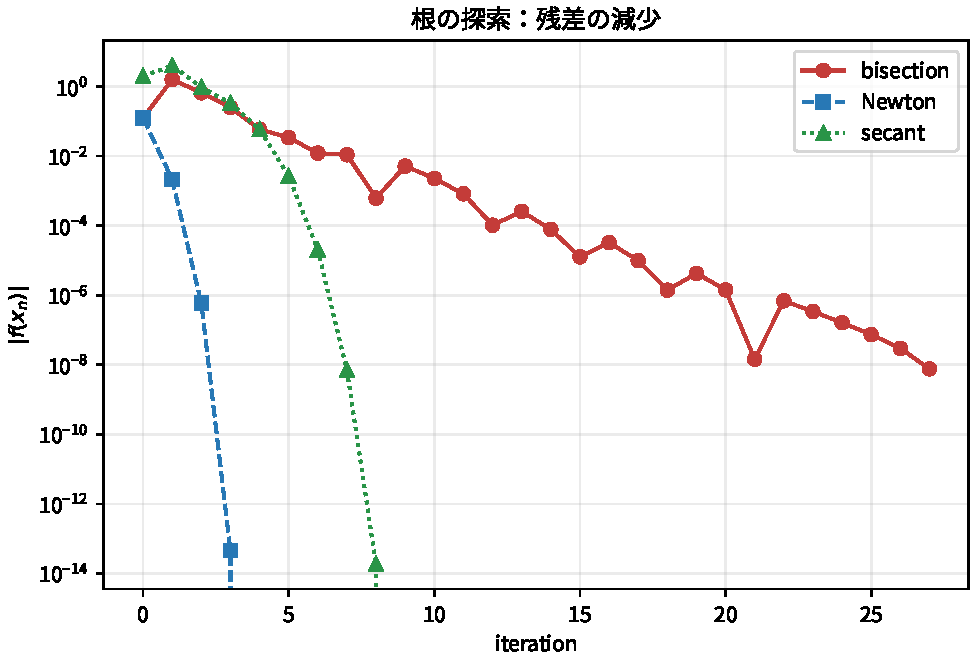
\includegraphics[width=.78\linewidth,height=48mm,keepaspectratio]{root_convergence.pdf}
  \par\small \(f(x)=x^3-x-2\)。二分法は\([1,2]\)、Newton法は\(x_0=1.5\)、割線法は\(x_0=1, x_1=2\)から開始。縦軸は\(|f(x_n)|\)。
\end{frame}

\begin{frame}[t]{停止条件を決める}
  反復を始める前に、許容誤差と最大反復回数を決める。
  \begin{itemize}
    \item 二分法：区間幅\(b-a\)または残差\(|f(m)|\)。
    \item Newton・割線法：残差\(|f(x_n)|\)を確認する。
    \item ステップ幅\(|x_{n+1}-x_n|\)も併せて使う。
    \item 最大反復回数に達したら、収束失敗として扱う。
  \end{itemize}
  \vfill
  \begin{lessonbox}
    表示桁数を増やしても、残差が小さくなるとは限らない。
  \end{lessonbox}
\end{frame}

\begin{frame}[t]{固定点反復}
  方程式を\(x=g(x)\)と書き直し、右辺を繰り返し計算する。
  \[
    x_{n+1}=g(x_n).
  \]
  \begin{itemize}
    \item 解\(x_*=g(x_*)\)の近くで\(|g'(x_*)|<1\)なら局所収束する。
    \item 同じ方程式でも、書き換え方で収束性が変わる。
    \item 収束後は\(|g(x)-x|\)を確かめる。
  \end{itemize}
\end{frame}

\begin{frame}[t]{緩和を加える}
  更新が振動する場合、前の値を混ぜて動きを抑える。
  \[
    x_{n+1}=x_n+\alpha\bigl(g(x_n)-x_n\bigr),\qquad 0<\alpha\leq1.
  \]
  \begin{itemize}
    \item \(\alpha=1\)：通常の固定点反復。
    \item \(0<\alpha<1\)：更新幅を小さくする。
    \item 緩和で安定になる場合があるが、収束は遅くなりうる。
  \end{itemize}
\end{frame}

\begin{frame}[t]{実習：講義資料の3関数}
  \[
    \begin{aligned}
      f(x)&=x^3-x-2,\\
      g(x)&=\cos x-x,\\
      h(x)&=\log x+x-3.
    \end{aligned}
  \]
  \begin{itemize}
    \item \(f,g,h\)：二分法で解く。\(h\)は\(x>0\)の区間を選ぶ。
    \item \(f,g,h\)：Newton法と割線法で解き、残差を比べる。
    \item \(g,h\)：固定点の形に書き直して解く。
  \end{itemize}
  \vfill
  \begin{lessonbox}
    \code{2026/week14/week14.ipynb}の演習セルは空欄。
  \end{lessonbox}
\end{frame}

\begin{frame}[t]{まとめと参考}
  \begin{itemize}
    \item 二分法は連続性と符号変化を使い、区間を確実に縮める。
    \item Newton法は導関数を使い、適切な初期値なら速く収束する。
    \item 割線法は導関数を差分で置き換える。
    \item 固定点反復では写し方と局所収束条件が重要。
    \item 近似根の残差と反復回数を確認する。
  \end{itemize}
  \vfill
  {\footnotesize
    野本拓也・是常隆・有田亮太郎『実践計算物理学』共立出版。\\
    SciPyの二分法：\url{https://docs.scipy.org/doc/scipy/reference/generated/scipy.optimize.bisect.html}}
\end{frame}

\end{document}
